% @Date:   2019-04-01 23:02:29
% @Last Modified by:   Discount

\documentclass[UTF8]{article}
    \author {刘林冬、齐向彤、徐宙}
    \title {基于拉格朗日松弛理论的非平衡博弈
费用分摊算法}
    \date{}
\usepackage{ctex}
\usepackage{amsmath}
\usepackage{geometry}
\geometry{a4paper,scale=0.8}
\usepackage{graphicx}
\usepackage{amssymb}
\begin{document}
    \maketitle
\begin{abstract}
针对核为空的合作博弈费用分摊问题,在满足大联盟稳定性条件下,本文研究了将分摊给所有局中人的总费用最大化的算法。此类问题的应用之一就是找到稳定大联盟所需的最低补贴费用。为求解此问题,我们提出了基于拉格朗日松弛理论的非平衡博弈费用分摊算法。与现有的基于线性松弛理论的算法相比,本文提出的算法可以得到更好结果,并且其适用范围也更加广泛。为证明该算法的有效性,本文研究了两种不同的设施选址博弈。结果表明,该算法不仅保证了新算法的效用,而且很大程度的拓展深化了费用分摊问题的研究广度与深度。

\end{abstract}

\begin{keywords}
关键词:博弈论、合作博弈、费用分摊、拉格朗日松弛、设施选址博弈
\end{keywords}

\section{引言}
合作博弈理论解决了多个独立决策人之间的合作问题。它在经济、金融、运筹学(OR)和电信等多个领域都有应用。在降低成本的应用中, (具有可转移效用的) 合作博弈可以大致表述为:有$n$个局中人,每个局中人都需要利用其资源以最小的费用完成既定的任务目标。为了降低总成本,有些(或所有)局中人可能会通过结盟的方式集中资源实现任务目标。所有局中人的集合被称为大联盟。主要的问题是如何以“公平”的方式分摊大联盟的费用,使得任何一位局中人不会退出。
定义费用分摊的“公平”有不同的方法,但是一个根本的概念就是联盟的稳定性。它要求分摊给每个联盟的成本 (分摊给联盟中每个局中人的成本之和)不超过联盟成员未加入联盟时的最低成本。另外,需要有一个要求分摊给所有局中人的总成本等于大联盟最低成本的预算平衡约束。合作博弈的核心是联盟的费用分配集满足(1)联盟稳定性和(2)预算平衡约束。如果至少存在一个这样的分配,那该博弈的核心就不为空,大联盟就是稳定的。目前已有许多方法可以判断各种合作博弈的核是否为空。
然而许多合作博弈问题都是空核。对于空核博弈,已经有人提出了用替换的概念来给出解决方案。其基本思想是松弛核心定义的两个条件之一。例如,松弛联盟稳定性的最小核概念。在最小核心概念中,分摊给每个联盟的费用不超过一个值$z$与联盟的最小成本之和,其中z是一个最小化的参数。
在另一个被称为{\em $\gamma$-core}的概念中,预算平衡约束被替换为$\gamma$预算平衡约束。$\gamma$预算平衡约束指分摊给所有局中人的总成本不小于$\gamma$乘以大联盟的最低费用,其中$0<\gamma\leq 1$。在数学领域{\em $\gamma$-core}等同于另一个概念{\em $\epsilon$-approximate core}。这一概念约束预算平衡,松弛联盟稳定性,使分配给每个联盟的成本之和不超过$(1+\epsilon)$倍的联盟的最低费用。总之,研究$\gamma$-core 或 $\epsilon$-approximate core的关键点是在具体的博弈中找到$\gamma$或$\epsilon$的连续边界。
在本文中,我们探究了$\gamma$-core。但与原文的关注点不同,对于由Caprara和Letchford提出的最优费用分摊问题(OCAP),我们设计了一种算法来精确计算任意给定博弈的最佳$\gamma$值,而不是只寻找$\gamma$的连续边界。特别地,OCAP尝试最大化分摊给所有局中人的总费用。正如Caprara和Letchford所指出的,这可以等价地看作计算在大联合政府下稳定社会最优状态的“费用”。在大联合政府中,代表社会福利的第三方愿意为大联合政府的稳定提供补助。在这里,第三方可能是政府机构,而参与者是一群私营公司。或者,第三方可能是一个大公司的总部,而参与者是不同的分公司。在这种情况下,OCAP的目标相当于最小化分配给所有局中人的总费用与大联盟总费用之间的差价,而这一差价则由第三方提供补助。
简单地说,找到OCAP的解至少有两个困难。首先,普通线性规划(LP)公式的约束数量随着局中人数量的增加而指数级增加,即$n$个参与者需要$2^n$个约束。其次,对于给定的费用分摊方案,仅验证其中一个LP约束是否被满足,就需要解NP-hard的优化问题。因此,直接用LP公式求解OCAP是非常困难的。
对于空核的合作博弈问题,首先想到的就是求解OCAP。然而,该问题一直未得到充分的研究,直到Caprara和Letchford提出了一个基于线性松弛理论的算法(LPB算法)。其基本思想是建立一个稳定的费用分摊方法。该方法可以得到大联盟成本的线性松弛下界。从理论上讲,LPB算法是可以最好地解决OCAP,但前提是识别并添加ILP公式中的所有“可分配”约束。然而,有时很难识别所有可分配的约束。如果没有多项式时间间隔算法来处理可分配约束的指数数量,即使在所有可分配的约束都可以被识别的情况下,LPB算法仍然是不适用的。例如,Caprara和Letchford(2010)研究的无根旅行商博弈。
本文基于拉格朗日松弛理论,提出了一个的新算法处理OCAP。该方法(LRB算法)虽然也试图找一种费用分摊方案使大联盟费用达到更低,但与LPB算法相比具有以下优势。
首先,它是一个通用算法,可以应用于比Caprara和Letchford所描述的更广泛的合作博弈。而且与LPB算法只能解决线性目标函数不同,新算法也适用于具有非线性目标函数的问题。
其次,由于拉格朗日松弛界不比松弛LP解提供的界差,对于模型相同的大联盟问题LRB算法可以找到比LPB算法更好的解。在一定程度上,这避免了LPB算法中识别所有“可分配”约束的要求。此外,即使在某些可找到所有可分配约束情况下,LRB算法仍然是有价值的。因为它可以为参与者提供可替代的最优费用分摊方案,从而提供更多的评估选择。
第三,在求解OCAP时,LRB算法利用分解的方法将原博弈问题分解为两个子博弈。子博弈1可以得到用闭型表示的最优解。子博弈2可以具有一些原博弈所缺的特性。在许多情况下与原博弈相比,子博弈中每个联盟产生的最小费用更容易计算。在某些情况下,子博弈的最优成本分配是多项式可解的,而原始博弈的最优成本分配不是多项式可解的。
最后,LRB算法是依赖于几十年来求解拉格朗日对偶问题的大量研究。在将它应用到OCAP时,我们可以充分利用各种加速收敛和生成更清晰界限的方法。这些结果可以在LRB算法的第一步中进行合并。

\section{文献综述}
自Shapley的开创性工作以来,合作博弈的研究一直在深入研究。与运筹学应用相关的领域最为突出,主要包括分配博弈、装箱博弈、线性生产博弈、最小生成树博弈、旅行商博弈、车辆路径规划博弈、库存博弈、生产外包博弈以及一些图形包装和覆盖博弈等。这些博弈的研究重点通常是核心的存在性。
本文以设施选址博弈为例。Kolen(1983)给出了一个早期的重要结果。他指出,对于无容量设施选址(UFL)博弈,局中人的最大分摊费用等于大联盟优化问题的经典LP松弛成本。后来,Goemans和Skutella(2000)在此基础上扩展了这一研究,并证明了在一些特殊的设施选址博弈中的核心非空,如地址在一条线上、一个循环和一个树形网络上。其他人也研究了这个问题的变形。如Puerto 等(2011, 2012)分别介绍了最小半径选址博弈和最小直径选址博弈。Xu and Yang (2009), Mallozzi (2011), Li等人(2013)研究了考虑各种成本要素的设施定位博弈,如服务安装成本,区域固定成本,以及凹形设施选址成本。
如前文所述,最小核是一种可用于处理空核博弈的松弛方法。Faigle等人(2000)指出,计算最小生成树博弈的最小核分配是NP-hard问题。Kern和Paulusma(2003)基于基数匹配博弈中最小核的多项式描述研究了核仁。Schulz和Uhan(2010)的研究表明求一个具有超模成本单机调度博弈的最小核值是弱NP-hard问题,并为计算最小核值的3-approximate算法(界为3)提供了方法。关于$\gamma$-core 和 $\epsilon$-approximate core,使用后者进行研究的更多。例如,Faigle等人(1998)提出了一种基于LP的算法,为Euclidean TSP得出了一个1/3- approximate core。Blaser和Ram(2008)提出了一种多项式时间算法,该算法可以在一个$(\log_2(n-1)-1)$ -approximate core中得到非对称TSP博弈的费用分摊方法。我们建议读者参考Jain和Mahdian(2007)的研究以对先前的概念进行更全面的回顾。
现在仅有几篇论文直接研究OCAP。Bachrach等人(2009)提出了问题—在稳定合作博弈中大联盟的前提下,如何确定补贴的最小值并且得到最小值合适的上、下界?之后,Meir 等人(2011)进行了类似的关于联合博弈中限制合作的研究。目前唯一解决OCAP的算法是由Caprara和Letchford(2010)提出的。他们提出了一种基于LP松弛和对偶理论的算法。在他们的方法中,通常需要通过引入具有特殊结构的约束来重新表达优化问题。详细内容将在下一节中介绍。

\section{正文前述}
可转移效用的合作博弈用二元向量$(V,c)$表示,其中$V = \{1,2,...,v\}$表示局中人集合,$c:S \rightarrow \mathbb{R}$表示特征函数,$S= 2^V \setminus \emptyset$ 表示局中人非空的联盟集合。特征函数为每个联盟$s\in S$分配了一个值$c(s)$,代表了$s$中的成员在合作时需要支付的最小总成本。本文研究的费用分摊问题是在$V$中的局中人之间分摊大联盟的成本$c(V)$使得任何一个小联盟的局中人都没有动机脱离大联盟。
一个博弈$(V,c)$的稳定费用分摊是一个向量$\alpha \in \R^{v}$,其满足联盟稳定性:$\sum_{k \in s} \alpha(k) \leq c(s),~ \forall s \in S$。理想中的费用分摊另外满足预算平衡约束:$\sum_{k \in V} \alpha(k) = c( V)$ 。博弈$(V,c)$的核心定义为:
\begin {equation*} \label{eqn:budgetbalance}
Core(V,c)=\{\alpha \in \R^{v}:\sum_{k \in s} \alpha(k) \leq c(s),\forall s \in S, \mbox{ and } \sum_{k \in V} \alpha(k) = c( V)\}.
\end {equation*}
众所周知,并不是每个博弈$(V,c)$都有非空的核心。要求解核心为空的博弈,我们的目标是找到一个稳定的费用分摊方案,尽可能多地接近大联盟成本$c(V)$。这就是最优费用分摊问题,定义如下:
\begin{eqnarray}\label{eqn:OCAP}
\begin{aligned}
\begin{split}
\max_{\alpha} \sum_{k \in V} \alpha(k)&\\
s.t. \sum_{k \in s} \alpha(k) \leq  c(s),~ \forall &s \in S.
\end{split}
\end{aligned}
\end{eqnarray}
通常很难直接求解$(\ref{eqn:OCAP})$,因为它包含一个指数级的约束条件,而且计算特征函数$c(s)$可能是NP -难问题。本文的重点是为OR博弈求得稳定的最优费用分摊方案。该类博弈的核心可能为空,特征函数由整数规划定义,是Caprara and Letchford (2010)研究的整数最小化(IM)博弈的推广。与只能使用ILP来定义特征函数的IM博弈不同,OR博弈允许使用非线性整数规划来定义特征函数。

\begin{Definition}\label{def2}
如果一个博弈$(V,c)$满足以下条件,则该博弈被称为OR博弈。\\
$~~\bullet$
正整数 $r$, $r'$ 和 $t$,\\
$~~\bullet$ 左边矩阵 $A \in \R^{r \times t}$ 和 $A' \in \R^{r' \times t}$,\\
$~~\bullet$ 右边矩阵 $B \in \R^{r \times v}$和 $B' \in \R^{r' \times v}$,\\
$~~\bullet$ 右边非负列向量 $D \in \R^{r}$ and $D' \in \R^{r'}$,\\
$~~\bullet$ 线性或非线性目标函数 $f(x)$,\\
$~~\bullet$ 对于所有$s \in S$,示性列向量 $\gamma^s \in \{0,1\}^v$满足:若 $k \in s$且 $\gamma_k^s=0$, 则 $\gamma_k^s=1$ 否则, $\forall k \in V$,\\
则特征函数$c(s)$用整数规划表示为:
\begin{equation}\label{eqn:orgc}
c(s) = \min_{x} \big\{ f(x):Ax \geq B\gamma^s + D, A'x \geq B'\gamma^s + D', x \in \{0,1\}^{t \times 1} \big\}.
\end{equation}
\end{Definition}

注意,在式(2)中,为方便使用拉格朗日松弛,约束被分为两部分。根据Caprara和chletford(2010)的研究,很容易证明每个OR博弈的非负列向量$D$和$D'$都具有次加性,即对于任意 $s_1,s_2 \in S$ ,$c(s_1 \cup s_2) \leq c(s_1) + c(s_2)$, 且 $s_1 \cap s_2 = \emptyset$。
IM博弈是OR博弈的一种特殊类型,它的特征函数$c(s) $是由整数线性规划表示为:
\begin{equation}\label{eqn:orgc1}
c(s) = \min_{x} \big\{ Cx:Ax \geq B\gamma^s + D, A'x \geq B'\gamma^s + D', x \in \{0,1\}^{t \times 1} \big\},
\end{equation}
其中$C$是$t$维行向量.我们用$c_{LP}(V)$ 表示(\ref{eqn:orgc1})中$c(V)$的LP下界,其中$x \in \{0,1\}^{t \times 1}$ 松弛为 ${\bf 0}\leq x \leq {\bf 1}$。
Caprara和Letchford(2010)给出了通过使用列生成、行生成或二者结合解决IM博弈的OCAP方法。,我们在online supplement中总结了这些方法的要点。列生成方法有一个简单的公式,但由于优化过程中需要极大的解空间,与其相关的定价问题通常很难处理。行生成方法需要通过识别被称为可分配约束的集合$\{ Ex \geq F\gamma\}$来重新确定ILP(3)。然后,通过求解仅具有可分配约束的LP松弛$c_{LP}^{EF}(V)=\min\{ Cx : Ex \geq F\gamma\}$得到费用分摊方案,其中总费用等于$c_{LP}^{EF}(V)$—为$c(V)$的下界之一。注意,$c_{LP}^{EF}(V)$可能与$c_{LP}(V)$不同。
对于IM博弈,LPB费用分摊方案的好坏很大程度上依赖于已确定的可分配的约束。从理论上讲,如果所有可分配的约束都能被识别和添加,LPB算法就能找到一个最优的稳定成本。然而,对于不同IM博弈,识别可分配约束的方法通常不同。对于一些可分配的约束,没有已知的多项式时间间隔算法又增加了计算的难度。尽管存在这些问题,LPB算法依然可以作为一种有效的启发式算法,在只添加可分配约束的子集的情况下,找到良好的稳定的费用分摊方案。

\section{4}




    \subsection{4.1} test2.


    \subsection{4.2} test2.

    \subsection{4.3}  test2.


\section{设施选址博弈的实现}
我们将在两种不同的设施位置博弈中说明LRB成本分配算法,即UFL博弈和非线性单源容量设施位置博弈。UFL博弈是利用LPB和LRB算法来计算最优成本分配的一种情况;此外,得到的UFL子博弈2是次模的,其核心成本分配可以在多项式时间内得到。NLCFL博弈具有不同的联合定义和非线性代价函数,显示了我们的LRB算法的全部能力。

  \subsection{UFL 博弈}\label{section:UFL}
在一个UFL博弈中,有一个双向网络图定义为 $G=(M,N,E)$, 其中 $M$ 为潜在工厂开设的集合,$N$ 为必须被服务顾客的集合,$E$ 为连接工厂和顾客所形成边的集合。每一个工厂潜在开设点 $i \in M$ 都有一个固定开启成本 $f_i$,并且每一条边 $(i,j) \in E$ 都有一个运输成本 $c_{ij}$。在UFL博弈中,顾客分享工厂开启和运输的成本,即在博弈中的参与者是顾客。我们在表中列出了在UFL中需要用到的记号。
Table~\ref{table:notationsUFL}.
\begin{table}[H]
\vspace{-2mm}
\tabcolsep=7pt
\small
\renewcommand\arraystretch{1.5}
\caption{\label{table:notationsUFL} Notation used in the UFL game}
\vglue5pt
\begin{tabular}[!h]{c c}
\hline
%\multicolumn{1}{c}{Symbol} &\multicolumn{1}{c}{Meaning}\\
%\cline{1-2}
\multicolumn{1}{c}{$M$} &\multicolumn{1}{l}{潜在设施位置集合, $M=\big\{1,2,...,m\big\}$.}\\
\multicolumn{1}{c}{$N$} &\multicolumn{1}{l}{顾客即博弈参与者集合, $N=\big\{1,2,...,n\big\}$.}\\
\multicolumn{1}{c}{$c_{ij}$} &\multicolumn{1}{l}{从设施 $i$ 到顾客 $j$ 的转移成本, $\forall i \in M, j \in N$.}\\
\multicolumn{1}{c}{$f_i$} &\multicolumn{1}{l}{设施 $i$ 开启的固定成本, $\forall i \in M$.}\\
\multicolumn{1}{c}{$s$} &\multicolumn{1}{l}{参与者联盟, $s \subseteq N$.}\\
\multicolumn{1}{c}{$\gamma^s$} &\multicolumn{1}{l}{Incidence 向量 $\big[ \gamma^{s}_1,\gamma^{s}_2,...,\gamma^{s}_{n}\big]^T$, 如果参与者 $j$ 在联盟 $s$ 中则有$\gamma^{s}_j=1$否则 $\gamma^{s}_j=0$}\\
\multicolumn{1}{c}{$v_i$} &\multicolumn{1}{l}{决策变量, 如果设施 $i$ 开启则有 $v_i=1$ 否则 $v_i=0$, $\forall i \in M$.}\\
\multicolumn{1}{c}{$u_{ij}$} &\multicolumn{1}{l}{决策变量, 如果参与者 $j$ 被设施 $i$ 服务则有$u_{ij}=1$ 否则 $u_{ij}=0$}\\
\multicolumn{1}{c}{} &\multicolumn{1}{l}{ $\forall i \in M$ and $j \in N$.}\\
\hline
\end{tabular}
\vspace{-3mm}
\end{table}

\begin{定义}\label{defi:ug}
UFL 博弈 $(N,c_{UFL})$ 的定义为,在集合 $N$ 中的顾客为参与者并且特征函数为 $c_{UFL}(s)$ 由如下的整数规划决定,

\begin{equation}\label{eqn:ugobj}
c_{UFL}(s) = \min_{v,u} \sum_{i \in M} f_iv_i + \sum_{i \in M} \sum_{j \in N} c_{ij}u_{ij}
\end{equation}
\begin{equation} \label{eqn:ugcon1}
s.t.~\sum_{i \in M} u_{ij} \geq \gamma_j^s, ~\forall j \in N,
\end{equation}
\begin{equation}\label{eqn:ugcon2}
u_{ij} - v_i \leq 0, ~\forall i \in M, j \in N,
\end{equation}
%\begin{equation}\label{eqn:ugcon3}
%u_{ij} \leq \gamma_j^s, ~\forall i \in M, j \in N
%\end{equation}
\begin{equation}\label{eqn:ugcon4}
v_i, u_{ij} \in \{0,1\}, ~\forall i \in M, j \in N.
\end{equation}
\end{definition}

在上述的整数规划中,目标函数 $(\ref{eqn:ugobj})$ 是为了最小化对于一个联盟 $s$ 中工厂开启和运输的总成本,限制条件 $(\ref{eqn:ugcon1})$ 需要在联盟 $s$ 中的每一位顾客被
服务,而限制条件 $(\ref{eqn:ugcon2})$ 确保了只有一个开启的工厂可以服务顾客。

整数规划 (\ref{eqn:ugobj})-(\ref{eqn:ugcon4}) 是对于一个无容量限制的设施选址问题的常规表达式。基于定义, 我们可以看到UFL博弈 $(N,c_{UFL})$ 是一个OR博弈 $(V,c)$ 其中 $V=N$,$c = c_{UFL}$。特别地,在 $c$ 中的决策变量 $x$ 现在变为在$c_{UFL}$ 中的 $[v;u]$, 并且矩阵 $C$, $A$, $A'$, $B$, $B'$, $D$, $D'$ 的具体表达式也可以通过用矩阵写出 $c_{UFL}$ 而得到。 特别地,$D$ 和 $D'$ 现在都是 $\textbf{0}$,所以博弈 $(N,c_{UFL})$ 是次可加的。这一点对于我们接下来要研究的 ULCFL 博弈来说也是正确的。

      \subsubsection{对于UFL博弈线性规划解的成本分配}
      \cite{Kolen1983FacilityLocationGame} 和 \cite{Goemans2000FacilityLocationGames} 证明了,对于一个UFL博弈,最大稳定成本分配值与 $c_{UFL}(N)$ 的LP下界重合。为了做进一步的分析,我们给出了使用 LPB 算法来计算最优稳定成本分配的更多细节。

      在 $c_{UFL}(s)$ 中,限制条件 $(\ref{eqn:ugcon1})$ 和 $(\ref{eqn:ugcon2})$ 已经是可分配的。通过加入可分配限制条件 $\{u_{ij} \geq 0:i \in M, j \in N\}$ 来松弛二元限制条件 (\ref{eqn:ugcon4}),我们可以得到一个对于大联盟最优解问题 $c_{UFL}(N)$ 的LP松弛如下:

      \begin{equation*}\label{eqn:lpugobj}
      c_{LP\_UFL}(N) = \min_{v,u} \sum_{i \in M} f_iv_i + \sum_{i \in M} \sum_{j \in N} c_{ij}u_{ij}
      \end{equation*}
      \begin{equation} \label{eqn:lpugcon1}
      s.t.~\sum_{i \in M} u_{ij} \geq \gamma_j^N, ~\forall j \in N,
      \end{equation}
      \begin{equation}\label{eqn:lpugcon2}
      v_i - u_{ij} \geq 0, ~\forall i \in M, j \in N,
      \end{equation}
      \begin{equation}\label{eqn:lpugcon3}
      u_{ij} \geq 0, ~\forall i \in M, j \in N.
      \end{equation}

      我们有顺序地对限制条件$(\ref{eqn:lpugcon1})$, $(\ref{eqn:lpugcon2})$ 和 $(\ref{eqn:lpugcon3})$ 分别从 $1$ 到 $n$, $n+1$ 到 $n+mn$ 和 $n+mn+1$ 到 $n+2mn$ 进行标号。对于 $c_{LP\_UFL}(N)$,我们考虑它的对偶线性规划。让 $\mu_k$ 为$c_{LP\_UFL}(N)$ 的第 $k$ 个限制条件所对应的对偶变量, 并且 $\mu^*$ 为对偶式的最优解。
      根据在附录中的行生成方法,我们有如下的引理:

      \begin{lemma}\label{lemma:lpbcaufl}
      对于一个 UFL 博弈,LPB 成本分配 $\alpha_{LP\_UFL}$ 由下式给出
      \begin{equation*}
      \alpha_{LP\_UFL}(j) = \mu_j^*, ~\forall j \in \big\{1,2,\ldots,n\big\},
      \end{equation*}
      是最优的, 同时总的共享成本为 $c_{LP\_UFL}(N)$.
      \end{lemma}

      我们记一种对于UFL博弈得到最优稳定成本分配的简单方式是直接解 $c_{LP\_UFL}(N)$ 并且通过计算限制条件的影子价格得到最优对偶变量。然而,解对偶线性规划有助于找到替代的最优解,因为在对偶LP有多个最优解的情况下,并不是所有的都对应于原始的影子价格。

      \subsubsection{对于UFL博弈拉格朗日松弛解的成本分配}
      接下来我们将演示如何应用LRB算法来获得UFL博弈的最优成本分配。我们将证明UFL博弈的子博弈2是次模的。我们还将通过计算实验表明,LRB算法所获得的该博弈的最优成本分配与LPB算法所获得的成本分配不同,从而为评价和比较提供更多的选择。

      在 $c_{UFL}(s)$ 中,我们加入了一系列新的限制条件
      \begin{equation}\label{eqn:UFLLRBC}
      \big\{ u_{ij} \leq \gamma_j^s: ~\forall i \in M, j \in N\ \big\},
      \end{equation}
      然后引入限制条件 $\{ \sum_{i \in M} u_{ij} \geq \gamma_j^s:j \in N \}$ 到加入了非负拉格朗日乘子 $\sigma$ 的目标函数中,从而得到UFL的拉格朗日特征函数。

      \begin{eqnarray*}\label{eqn:LRPGCF}
      \begin{aligned}
      \begin{split}
      c_{LR\_UFL}(s;\sigma) = \min_{v,u} \sum_{i \in M} f_iv_i + &\sum_{i \in M} \sum_{j \in N} \big(c_{ij} - \sigma_{j}\big)u_{ij} + \sum_{j \in N} \sigma_j \gamma_j^s\\
      s.t.~u_{ij} - v_i \leq 0,&~\forall i \in M, j \in N,\\
      u_{ij} \leq \gamma_j^s,~\forall i& \in M, j \in N,\\
      v_i,u_{ij} \in \{0,1\},~&\forall i \in M, j \in N.
      \end{split}
      \end{aligned}
      \end{eqnarray*}

      约束条件 $(\ref{eqn:UFLLRBC})$ 的增强是为了加强 $c_{UFL}(s)$ 的拉格朗日下界,这有可能因此得到更好的LRB成本分配。。
      它禁止设置 $u_{ij'}=1$ 对于任何不在联盟s中的参与者,即使计算$c_{LR\_UFL}(s;\sigma)$时,系数 $c_{ij'}- \sigma_{j'}<0$。
      很容易看出 $(\ref{eqn:UFLLRBC})$ 的增强只相当于在目标函数 $c_{LR\_UFL}(s;\sigma)$ 中替换术语 $\sum_{i \in M} \sum_{j \in N} \big(c_{ij} - \sigma_{j}\big)u_{ij}$ by $\sum_{i \in M} \sum_{j \in s} \big(c_{ij} - \sigma_{j}\big)u_{ij}$。

      在算法 \ref{algolrb}下,一般的LRB成本分配算法对于任何 $s \in S$ 和非负拉格朗日乘子 $\sigma$, 我们可以分解 $c_{LR\_UFL}(s;\sigma)$ 为 $c_{LR1\_UFL}(\ \cdot \ ;\sigma)$ 和 $c_{LR2\_UFL}(\ \cdot \ ;\sigma)$ 使得 $c_{LR\_UFL}(s;\sigma) = c_{LR1\_UFL}(s;\sigma) + c_{LR2\_UFL}(s;\sigma)$, and define UFL sub-game 1 $\big(N,c_{LR1\_UFL}(\ \cdot \ ;\sigma)\big)$ and UFL sub-game 2  $\big(N,c_{LR2\_UFL}(\ \cdot \ ;\sigma)\big)$.

      对于UFL的子博弈1,它的特征函数是

      \begin{eqnarray}\label{eqn:UFLCFsub1}
      \begin{aligned}
      \begin{split}
      c_{LR1\_UFL}(s;\sigma) = \sum_{j \in N} \sigma_j \gamma_j^s.
      \end{split}
      \end{aligned}
      \end{eqnarray}

      根据引理 $\ref{lemma:lr1core}$,最优稳定成本分配 $\alpha_{LR1\_UFL}^{\sigma}$ 位于由 $\alpha_{LR1\_UFL}^{\sigma}(j) = \sigma_j$ $j \in N$ 给出的博弈 $\big(N, c_{LR1\_UFL}(\ \cdot \ ;\sigma)\big)$ 的核中。

      对于UFL的子博弈2,它的特征函数为
      \begin{eqnarray}\label{eqn:UFLCFsub2}
      \begin{aligned}
      \begin{split}
      c_{LR2\_UFL}(s;\sigma) = \min_{v,u} \sum_{i \in M} &f_iv_i + \sum_{i \in M} \sum_{j \in N} \big(c_{ij} - \sigma_{j}\big)u_{ij}\\
      s.t.~u_{ij} - v_i \leq 0,&~\forall i \in M, j \in N,\\
      u_{ij} \leq \gamma_j^s,~\forall i& \in M, j \in N,\\
       v_i,u_{ij}, \in \{0,1\},~&\forall i \in M, j \in N.
      \end{split}
      \end{aligned}
      \end{eqnarray}
      为了解 $c_{LR2\_UFL}(s:\sigma)$,我们可以将其分解为各种条件,并且得到一个闭式的由下式给出的最优目标函数值 $c_{LR2\_UFL}(s;\sigma) = \sum_{i=1}^m \min \big\{0,f_i+\sum_{j \in s} \min \{0,c_{ij}-\sigma_j\}\big\}$ 。

      \begin{lemma}\label{lemma:UFLSubmodular}
      UFL sub-game 2 $\big(N,c_{LR2\_UFL}(\ \cdot \ ;\sigma)\big)$ is submodular.
      \end{lemma}
      {\scshape Proof.}
      Denote $a$ and $b$ as two players in $N$. To show the submodularity, we need to prove that, for any coalition $s \in N\setminus \big\{a,b\big\}$,
      \begin{equation}\label{ll14}
      c_{LR2\_UFL}(s \cup \{a\}; \sigma) - c_{LR\_UFL2}(s;\sigma) \geq c_{LR2\_UFL}(s \cup \big\{a,b\big\};\sigma) - c_{LR2\_UFL}(s \cup \{b\};\sigma).
      \end{equation}

      对于每一个 $i\in M$,令 $\Delta_i(s;\sigma) = \min \{0, f_i + \sum_{j \in s} \min \{0, c_{ij} - \sigma_j\} \}$。为了证明 (\ref{ll14}),足够证明

      \begin{equation}\label{eqn:submodularufl}
      \Delta_i(s;\sigma) + \Delta_i(s \cup \{a,b\};\sigma) \leq \Delta_i(s \cup \{a\};\sigma) + \Delta_i(s \cup \{b\};\sigma), ~\forall s \in N\setminus\big\{a,b\big\}. \end{equation}

      令 $\rho(x)=\min\{0,x\}$,并且定义 $x_{\hat{s}}= f_i + \sum_{j \in \hat{s}} \min \{0, c_{ij} - \sigma_j\}$ for each $\hat{s}\in \{s,s\cup\{a\},s\cup\{b\},s\cup\{a,b\}\}$。
      可以看出 $x_s+x_{s\cup\{a,b\}} = x_{s\cup \{a\}}+x_{s\cup\{b\}}$, 和 $x_{s\cup\{a,b\}}\leq \min\{x_{s\cup \{a\}},x_{s\cup\{b\}}\}\leq  \max\{x_{s\cup \{a\}},x_{s\cup\{b\}}\} \leq x_{s}$.
      因此,既然 $\rho(x)$ 是一个关于 $x$ 的凹函数,我们有

      \begin{eqnarray*}
        \rho(x_s) + \rho(x_{s\cup \{a,b\}}) \leq \rho(x_{s\cup\{a\}}) + \rho(x_{s\cup \{b\}}),
      \end{eqnarray*}
      从中我们可以直接得到 (\ref{eqn:submodularufl}),并且完成了引理的证明。
      \hfill\Halmos

      由于UFL子博弈2的次模性,我们能够很容易地计算它的核成本分配,记为 $\alpha_{LR2\_UFL}^{\sigma}$,通过子博弈章节中的贪心算法。在最优拉格朗日乘子 $\sigma^*$ 下,我们可以得到由 $\alpha_{LR\_UFL}^{\sigma^*} = \alpha_{LR1\_UFL}^{\sigma^*} + \alpha_{LR2\_UFL}^{\sigma^*}$ 给出的最优UFL的LRB成本分配。
      既然UFL的子博弈1和子博弈2都有非空核,通过定理 \ref{thm:lagcostallocation1} 最优LRB成本分配值达到了拉格朗日下界 $c_{LR\_UFL}(N;\sigma^*)$,即不小于LP的下界 $c_{LP\_UFL}(N)$。

      下面的定理说明了UFL LRB成本分配的最优性,并揭示了LRB和LPB成本分配的等价性。

      \begin{theorem}\label{lemma:lpbequallrbufl}
      对于一个UFL博弈, LRB 的成本分配 $\alpha_{LR\_UFL}^{\sigma^*} = \sigma^* + \alpha_{LR2\_UFL}^{\sigma^*}$ 是最优的。 并且, LRB 成本分配集和 LPB 成本分配集都包含所有最优UFL成本分配。
      \end{theorem}
      {\scshape Proof.}

      对于UFL博弈,我们首先证明了LRB的成本分配是最优的。如前所述,最优LRB成本分配值达到拉格朗日下界 $c_{LR\_UFL}(N;\sigma^*)$,其不小于LP下界 $c_{LP\_UFL}(N)$。
      我们知道对于UFL博弈的LP下界等于最大总共享成本 \citep{Kolen1983FacilityLocationGame,Goemans2000FacilityLocationGames}。因此,LRB成本分配一定是一个最优UFL成本分配,并且 $c_{LR\_UFL}(N;\sigma^*)=c_{LP\_UFL}(N)$。

      然后,我们证明了LRB成本分配集和LPB成本分配集都包含所有的最优UFL成本分配。众所周知,LPB成本分配集由所有最佳UFL成本分配\citep{Goemans2000FacilityLocationGames}组成。这意味着每个LRB成本分配必须属于LPB成本分配集。因此,仍然需要证明,每个LPB成本分配都属于LRB成本分配集。

      考虑到每一个LPB成本分配 $\alpha_{LP\_UFL}(j)=\mu^*_j$ for $j \in N$,这里 $\mu^*$ 和 一些 $\delta^*$ 构成一个最优解对于下面的关于 $c_{LP\_UFL}(N)$ 的对偶问题:

      \begin{eqnarray*}
      \begin{aligned}
      \begin{split}\label{eqn:UFLLRdual1}
       \max_{\mu,\delta} \sum_{j \in N}&\mu_j\\
      s.t.~\sum_{j \in N}\delta_{ij} = f_i&, ~\forall i \in M,\\
      \mu_j - \delta_{ij} \leq c_{ij}, ~\forall i& \in M, j \in N,\\
       \mu_j \geq 0, \delta_{ij} \geq 0,~\forall &i \in M, j \in N.
      \end{split}
      \end{aligned}
      \end{eqnarray*}

      对每一个 $i\in M$, 可以看出 $f_i = \sum_{j\in N}\delta^*_{ij}$,并且 $\delta^*_{ij}\geq \max\{0,\mu^*_j-c_{ij}\}$ 对于 $j \in N$,这表明 $f_i \geq \sum_{j\in N}\max\{0,\mu^*_j-c_{ij}\}=-\sum_{j\in N}\min\{0,c_{ij}-\mu^*_j\}$。
      因此,我们有
      \begin{eqnarray}
        \min\{0,f_i + \sum_{j\in N}\min\{0,c_{ij}-\mu^*_j\}\} =0, \mbox{ for each $i\in M$.} \label{eqn:cost}
      \end{eqnarray}
      既然 $c_{LR2\_UFL}(N;\sigma)=\sum_{i=1}^{m}\min\{0,f_i+\sum_{j\in N}\min\{0,c_{ij}-\sigma_{j}\}\}$ 对于任何非负 $\sigma$ 成立,由 (\ref{eqn:cost}) 我们有 $c_{LR2\_UFL}(N;\mu^*) = 0$。
      同时加上 $c_{LR1\_UFL}(N;\mu^*)=\sum_{j\in N}\mu^*_j$ 该式,表明 $c_{LR\_UFL}(N;\mu^*) = \sum_{j\in N}\mu^*_j = c_{LP\_UFL}(N)=c_{LR\_UFL}(N;\sigma^*)$。
      因此 $\mu^*$ 是一个最优拉格朗日乘子。
      由此产生的LRB成本分配如下:$\alpha^{\mu^*}_{LR\_UFL}(j) = \mu^*_j + \alpha^{\mu^*}_{LR2\_UFL}(j)$ for $j \in N$。
      注意到对于每一个 $s\in S$,因为 $c_{LR2\_UFL}(s;\mu^*)\leq 0$ 和 $c_{LR2\_UFL}(s;\mu^*)\geq c_{LR2\_UFL}(N;\mu^*)=0$,我们有 $c_{LR2\_UFL}(s;\mu^*)=0$,这将得到 $\alpha^{\mu^*}_{LR2\_UFL}(j) = 0$ 对于所有 $j\in N$。
      因此我们得到 $\alpha^{\mu^*}_{LR\_UFL} = \mu^*$,表明每一个LPB成本分配 $\mu^*$ 属于LRB成本分配集。这就完成了定理
      \ref{lemma:lpbequallrbufl} 的证明。
      \hfill\Halmos

      \subsubsection{替代最优稳定成本分配}\label{section:uflcomputation}
      对于一个UFL博弈,我们知道每一个最优成本分配对应于一个LPB解,它必须是对偶式 $c_{LP\_UFL}(N)$ 的所有基本最优解的凸组合。 然而,只应用一般的LP求解方法于 对偶式 $c_{LP\_UFL}(N)$ 是很难得到所有基本最优解的。

      通过 \ref{lemma:lpbequallrbufl}, 我们知道LRB算法提供了对于UFL博弈的一种替代最优成本分配。所获得的LRB解有可能被排除在一般LP求解产生的LPB解之外。我们通过下面的例子来说明这一点。

      \begin{figure}[H]
      \centering
      \vspace{-0.1em}
      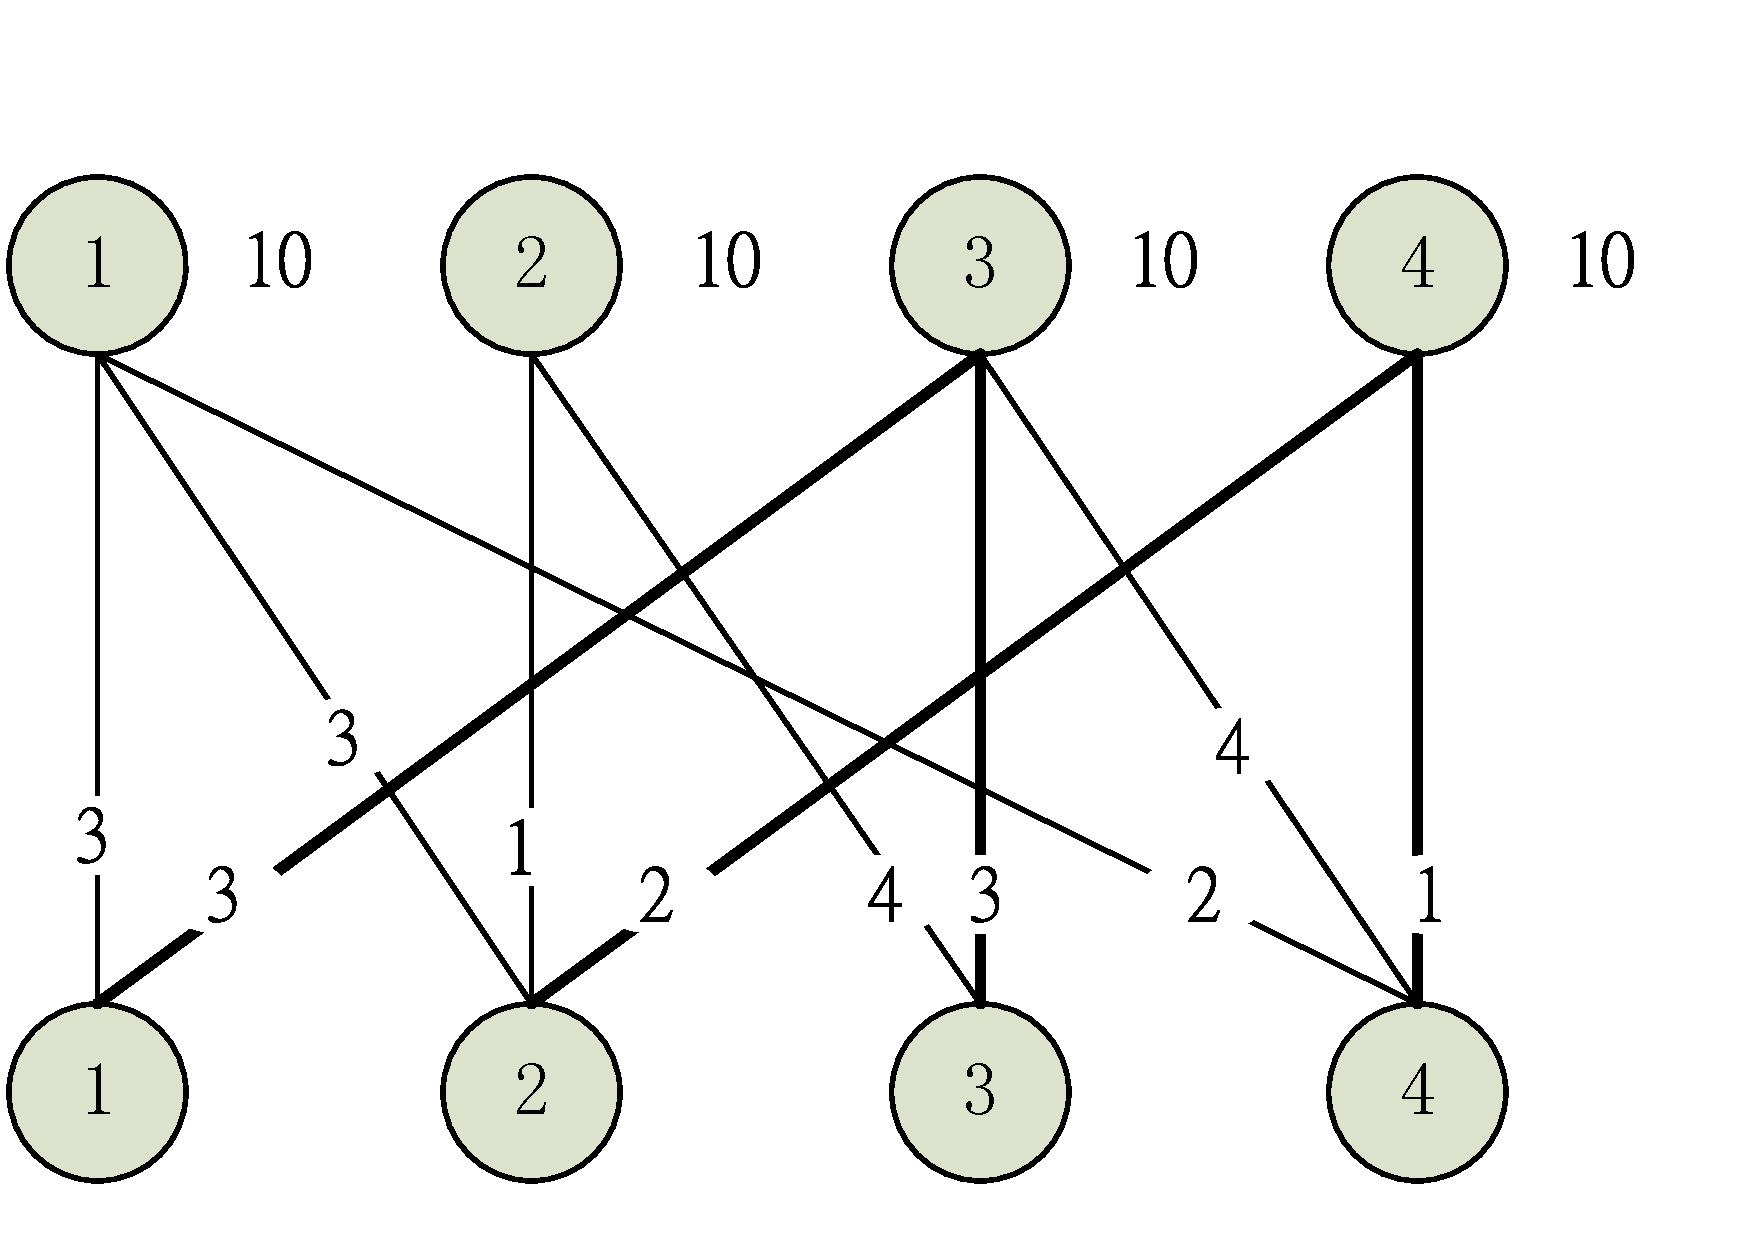
\includegraphics[width=0.5\textwidth]{figure-1.pdf}
      \caption{\label{figure:exampleUFL} UFL 博弈的一个例子}
      \vspace{-3mm}
      \end{figure}

      在图\ref{figure:exampleUFL}中所示的UFL博弈中,这里有四个设施和四个参与者。每一个设施有一个固定的启用成本10。在连接线上的数字代表从设施到参与者的运输成本。对于大联盟的一个最优解是开启设施3和4,并且画粗的连接线是最优路径。因此,大联盟所需要的成本是 10+10+3+3+2+1=29。

      在这个例子中,我们使用了两种 LP 求解方法,单纯形法和内点法,分别在 MATLAB 发行版本 2011a上计算LPB分配。
      表 \ref{table:UFLCA} 显示了在不同方法下的每一个参与者需要承担的成本。


      \begin{table}[H]
      \vspace{-2mm}
      \centering
      \tabcolsep=4pt
      \small
      \renewcommand\arraystretch{1.5}
      \caption{\label{table:UFLCA} 不同方法下的最优稳定UFL成本分配}
      \vglue5pt
      \begin{tabular}[!h]{c c c c c c c c c c c c c}
      \hline
      \multicolumn{1}{c}{方法}
      &\multicolumn{1}{c}{}
      &\multicolumn{1}{c}{参与者 1}
      &\multicolumn{1}{c}{}
      &\multicolumn{1}{c}{参与者 2}
      &\multicolumn{1}{c}{}
      &\multicolumn{1}{c}{参与者 3} &\multicolumn{1}{c}{}
      &\multicolumn{1}{c}{参与者 4}	&\multicolumn{1}{c}{}
      &\multicolumn{1}{c}{总共享成本}\\
      \hline
      单纯形法	& &5.00	& &6.50	& &8.50	& &6.50	&	&26.5	&\\
      内点法	& &6.58	& &6.50	& &8.50	& &4.92	&	&26.5	&\\
      LRB	& &6.87	& &6.50	& &8.50	& &4.63	&	&26.5	&\\
      \hline
      \end{tabular}
      \vspace{-3mm}
      \end{table}

      实例表明,LRB算法可以产生不同于一般LP方法的最优稳定成本分配。
      LRB解超出了两个LPB解的凸组合范围。
      这说明了LRB算法在提供替代成本分配方面的价值。

      为了研究LRB算法在一般设置下的能力,我们测试了由 \cite{Benchmark} 开发的30个无容量限制的设施位置基准实例,所有实例均有 $ M=N=100$。我们在一台Windows7 个人电脑上进行了所有的计算实验,该电脑的CPU型号为英特尔酷睿i7-2600,主频3.4GHz和内存为16G。所有算法均在Matlab 2011a版本中实现。
      在30个实例中,有22个实例的LRB解超出了两个LPB解的凸组合范围。
      同样,这显示了LRB算法在计算上寻找替代最优稳定成本分配方面的价值,即使在LPB成本分配显示为最优的情况下也是如此。

    \subsection{NLCFL}


      \subsubsection{LRB}

      \subsubsection{计算结果}

\section{结论}
本文的研究重点是核心可能为空的合作博弈。我们提出一个通用算法来计算得到一个最优的稳定费用分摊方案,使其在满足联盟的稳定性的条件下尽可能地覆盖大联盟的成本。在以往地研究中,这类问题主要通过LP松弛和对偶理论求解。我们采用与其不同的拉格朗日松弛理论求解。该方法的拉格朗日松弛下界不仅比现行松弛下界更具有竞争力,还打破了依赖于可分配约束和线性目标函数的局限。在两种代表典型的设施选址博弈应用该算法,结果表明该算法能够为这些博弈提供近乎最优的费用分摊方案,优于现有的LPB算法。


\end{document}
